\documentclass[letterpaper,11pt]{article}

\usepackage{fullpage,amsmath,amsfonts,latexsym,xcolor,clrscode3e}
\usepackage{graphicx}
\usepackage{amsthm}
\usepackage{hyperref}
\usepackage{fullpage}
\usepackage[ruled,vlined,linesnumbered]{algorithm2e}

\graphicspath{ {./images/} }

\newcommand{\re}{{\mathbb{R}}}
\newcommand\numberthis{\addtocounter{equation}{1}\tag{\theequation}}
\newcommand{\floor}[1]{\lfloor {#1} \rfloor}
\newcommand{\ceil}[1]{\lceil {#1} \rceil}
\newcommand{\paren}[1]{\left( {#1} \right)}
\newenvironment{solution}{\color{black} }{}

\newcommand{\nats}{\mathbb{N}}

\newcommand{\comment}[1]{$\rhd$\ {\small\sf #1}}

\newtheorem{theorem}{Theorem}
\newtheorem{claim}[theorem]{Claim}
\newtheorem{lemma}[theorem]{Lemma}
\newtheorem{problem}{Problem}


\begin{document}
{\noindent\large
{\em Introduction to Analysis of Algorithms} \hfill \today\\
Boston University \hfill CS 330\\
Professor  Adam Smith, Dora Erdos \hfill Fall 2020\\}
\vspace{1pt}
\hrulefill\vspace{3mm}
\begin{center}
{\LARGE\bf Homework 4}\\
{\bf Due Wednesday, September 30 at 11:59 PM}
\end{center}

\begin{center}
    \color{teal}
   Student: Justin DiEmmanuele \\
    Collaborators: Shilpen Patel, George Padavick, Matthew Gilgo
\end{center}


\section*{Homework Guidelines}

\paragraph{Collaboration policy} Collaboration on homework problems, with the exception of
programming assignments and reading quizzes, is permitted, but not encouraged.
If you
choose to collaborate on some problems, you are allowed to discuss
each problem with at most 5 other students currently enrolled in the
class.
Before working with others on a problem, you should think about it
yourself for at least 45 minutes. Finding answers to problems on the
Web or from other outside sources (these include anyone not enrolled
in the class) is strictly forbidden.

{\em You must write up each problem solution by yourself without
assistance, even if you collaborate with others to solve the
problem.} You must also identify your collaborators. If you did not
work with anyone, you should write "Collaborators: none." It is a
violation of this policy to submit a problem solution that you
cannot orally explain to an instructor or TA.

\paragraph{Solution guidelines} For problems that require you to provide an algorithm, you must give the following:
    \begin{enumerate}
\item  a precise description of the algorithm in English and, if helpful, pseudocode,
\item a proof of correctness,
\item an analysis of running time and space.
\end{enumerate}
You may use algorithms from class as subroutines. You may also use any facts that we proved in class.


You should be as clear and concise as possible in your write-up of
solutions. 

A simple, direct analysis is worth more points than a
convoluted one, both because it is simpler and less prone to error and
because it is easier to read and understand. Points might be
subtracted for illegible handwriting and for solutions that are too
long. Incorrect solutions will get from 0 to 30\% of the grade,
depending on how far they are from a working solution. Correct
solutions with possibly minor flaws will get 70 to 100\%, depending on
the flaws and clarity of the write up.

\newpage 
\begin{enumerate}


\item 
({\bf Unique simple path (15 pts)}) Given a {\bf directed} graph $G=(V,E)$, vertex $s$ has \emph{unique simple paths to all vertices} if for every $v\in V$ that is reachable from $s$, there is at most one simple path from $s$ to $v$ (Recall that a path is simple if all vertices on the path are distinct). 

The figure below gives example graphs and points out pairs of vertices that do and do not have unique paths. Go over the examples to make sure you understand the definition.


\begin{enumerate}
    \item For each of the following types of graphs, is it the case that in every graph of that type, every vertex $s$ has a unique simple paths to all reachable vertices? For each type of graph, give either a short proof (one or two sentences), if yes,  or a counterexample, if no.
        \begin{enumerate} 
        \item Cycles\footnote{A directed graph on $n$ vertices with directed edges of the form $(i,i+1)$ for $i=1,...,n-1$ and the edge $(n,1)$.}
            \begin{itemize}
                \color{teal}
                \item \textbf{Yes}
                \item A cycle is a sequence of \textbf{unique} nodes that cycles 
                    back to where it began as defined in section 3.1 of 
                    \textit{Algorithm Design}. If all the nodes in the sequence 
                    are unique than the edges between them are unique. Since
                    all the edges in the graph are involved in the cycle, there 
                    must be a simple unique path to all vertices. If there was
                    not, there would be a sub cycle in the graph.
            \end{itemize}
        \item DAGs (directed acyclic graphs)
            \begin{itemize}
                \color{teal}
                \item \textbf{No}
                \item The following counterexample is a DAG as it has no cycles 
                    but it also has \textbf{two} simple paths from 1 to 3.

                    \begin{figure}[htpb]
                        \centering
                        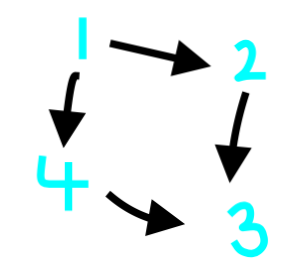
\includegraphics[width=0.2\textwidth]{1aii.png}
                        \caption{1.a.ii Counterexample}
                        \label{fig:1b}
                    \end{figure}    
            \end{itemize}

        \item Trees
            \begin{itemize}
                \color{teal}
                \item \textbf{Yes}
                \item  Any node pair with two paths between them must have a node 
                    in the path that has two edges leading into it and another
                    node in the path must have two edges leading out of it. This
                    is impossible because every node in a tree has one parent.
            \end{itemize}
        \item Strongly connected graphs
            \begin{itemize}
                \color{teal}
                \item \textbf{No}
                \item The following figure shows a counterexample. The graph 
                    is a strongly connected directed graph as there are paths
                    to and from each set of vertices. There are two paths from
                    1 to 4 - (1, 2, 4) and (1, 4).

                    \begin{figure}[htpb]
                        \centering
                        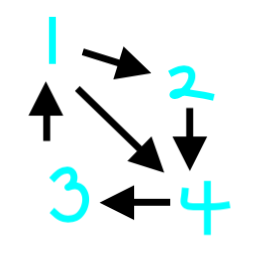
\includegraphics[width=0.2\textwidth]{1aiv}
                        \caption{1.a.iv Counterexample}
                        \label{fig:1aiv}
                    \end{figure}
            \end{itemize}
        \end{enumerate}
        
        \newpage
    \item Give an efficient algorithm that takes a directed graph $G$ and a vertex $s$ as input and checks whether $s$ has unique simple paths to all other vertices reachable from $s$. Your algorithm should output ``no'' if at least one vertex $v$ has more than one path from $s$ to $v$; otherwise it should output ``yes", together with  a tree of paths from $s$ to each reachable vertex in $G$.  For full credit, it should run in $O(m+n)$ time \emph{[Hint: Use DFS. Think about different kinds of non-tree edges.]}.
    \begin{itemize}
        \color{teal}
        \item \textbf{A precise description of the algorithm in English and, if helpful,
            pseudocode}

        \begin{itemize}
            \color{teal}
            \item To achieve the desired result, a slight modification will be 
                made to the DFS algorithm presented in the CS330 lecture. The 
                code presented in lecture is in black and the changes are in 
                teal.

        \color{black}

        \begin{algorithm}[H]
            \color{teal}
            \caption{UniqueSimplePaths(G, s)} 
            \KwIn{$G$ A graph in adjacency list form}
            \KwIn{$s$ source node to look for unique simple paths}
            $output = "Yes"$\;
            \For{each $u$ in $G.V$}{
                $u.color = WHITE$
            }
            $time = 0$ \;
            $DFS-Visit\left( G, s \right) $ \;
            \KwOut{$output$}
        \end{algorithm}

        \color{black}
        \begin{algorithm}[H]
            \caption{DFS-Visit(G, u)} 
            \KwIn{$G$ A graph in adjacency list form}
            \KwIn{$u$ edge to visit}
            $time = time + 1$ \;
            $u.d = time$ \;
             $u.color = gray$ \;

            \For{each $v$ in $G.Adj[u]$}{
                \If{$v.color = WHITE$}{
                    $v.p = u$ \;
                    $DFS-Visit(G, u)$
                }
                \color{teal}
                \uElseIf{$v.color = BLACK$}{
                    $output = "No"$
                }
                \color{black}
            }
            $u.color = Black$ \;
            $time = time + 1$ \;
            $u.f = time$ \;

        \end{algorithm}

        \color{teal}
        From the lecture, the node label of white means a node has not yet been 
        explored, Grey means the node has been discovered, and black means the
        node has been finished. The main thing we need to check if there is more
        than one simple, unique path to a node is to know if we come across a
        finished (Black) node when exploring another node. We only care about
        paths from the source node, so we only explore from there. This 
        allows us to not have to worry about cross edges. 

        \end{itemize}

    \color{teal}
    \item \textbf{A proof of correctness}
            \begin{itemize}
                \item Our claim is that if the DFS tree is exploring a node and comes 
                    across a finished (black) node, the edge it is exploring creates 
                    a second simple path.
                \item If we find a finished node $a$ while exploring node $b$, 
                    we know that node $a$ is not an ancestor of $b$.  
                    \begin{itemize}
                        \item We know this because if $a$ is an 
                            ancestor of $b$ it would still be in process of 
                            exploration. DFS goes deep before going wide. Any
                            node currently being explored has all it's ancestors
                            as unfinished. 
                        \item We care if $a$ is an ancestor of $b$ because if a
                            non-tree edge is to an ancestor of itself it can
                            not violate the unique simple path condition. The 
                            path it would create is not simple as node $a$ would
                            be repeated.
                    \end{itemize}
                \item We will not see cross edges since we are only running BFS 
                    from the source node. This means we do not have to worry 
                    about cross edges. Cross edges would have nothing to do with
                    simple paths from the source.
                \item Any remaining non-tree edges are either forward edges or
                    edges to a non-ancestor family member like an uncle. Edges 
                    of this type open up a second simple path to the finished 
                    node. Since the node is not an ancestor there must be a split
                    where the two paths taken allow for both paths to be simple.
            \end{itemize}
    \item \textbf{An analysis of running time and space}
        \begin{itemize}
            \item  As the only changes to the algorithm are constant time 
                comparisons, the running time and space will be the same as for
                normal DFS.
            \item Running time is $O\left( n + m \right) $ where $n$ is the 
                number of nodes in the graph and $m$ is the number of edges.
            \item Space complexity is $O\left( n + m \right) $ as we must 
                maintain the adjacency list graph representation.
        \end{itemize}

    \end{itemize}

\end{enumerate}

%\vfill

%\begin{center}
  %  \includegraphics[width=\columnwidth]{homework/homework 4/simple_path_examples.pdf}
%\end{center}


\newpage 
\item({\bf Lazy Hiker (10 pts)}) Suppose you are planning a hike in a forest with many paths. You want to start and end at the parking lot without visiting the same area of the forest twice. In addition, you get lost easily, so you want to choose the hike with the least possible number of trail intersections. 

You have a map, which you can interpret as a graph $G$: each vertex is a trail intersection (or start/end point) and each edge is a section of trail between two intersections. Note that $G$ is undirected.

Write an efficient algorithm that takes as input a graph $G = (V,E)$ and a ``parking lot vertex'' $p$ and outputs the a loop hike (starting and ending at $p$) that visits the smallest possible number of vertices while never covering the same trail segment twice. If there are no such loop hikes, your algorithm should output ``no loops from $p$''. For full credit, your algorithm should run in $O(n+m)$ time. See example graphs and correct outputs below.

\emph{Hint 1:} Run BFS starting from $p$ and divide the BFS tree into subtrees rooted at the  children of $p$. For each vertex $v$, figure out and store the subtree that it is part of. 

\textit{Hint 2:} The following questions may help you get thinking in the right direction. Do not hand these in. 
\begin{itemize}
    \item Prove that if you run BFS on an undirected graph, for every non-tree edge $(u,v)$ either $u$ and $v$ are in the same BFS layer, or $u$ and $v$ are off by one layer (e.g. $u$ is in layer $k$ and $v$ is in layer $k\pm1$)
    \item Non-tree edges create cycles. What do the numbers of the layers of the endpoints tell you about the length of the cycle and edge creates?
\end{itemize}

\begin{itemize}
    \color{teal}
    \item \textbf{A precise description of the algorithm in English and, if 
        helpful, pseudocode}

        \color{black}
        \begin{algorithm}[H]
            \color{teal}
            \caption{LazyHiker(G, s)} 
            \KwIn{$G$ A graph in adjacency list form}
            \KwIn{$s$ source node to look for the shortest cycle}
            $discovered[] =$ empty list \;
            $discovered[s] = True$ \;
            $nodes\_by\_layer[] =$ empty list length n\;
            $nodes\_by\_layer.append([s])$ A list containing s \;
            $layer\_counter = 0$ \;

            $subtree\_tracker =$ empty list to store which subtree each node is in \;

            \While{$len\left( nodes\_by\_layer[layer\_counter] \right) > 0$}{
                \For {$node$ in $nodes\_by\_layer[layer\_counter]$} {
                    \For {$adj\_node$ in $G.adj[node]$ }{
                        \If {$layer\_counter = 0$}{
                            $subtree\_tracker[adj\_node] = adj\_node$
                        }
                        \If{not $discovered[adj\_node]$ }{
                        $discovered[adj\_node] = True$ \;
                        $adj\_node.parent = node$ \;
                        $nodes\_by\_layer[layer\_counter + 1].append(adj\_noe)$\;
                            \If{$layer\_counter > 0$}{
                                $subtree\_tracker[adj\_node] = subtree\_tracker[node]$
                            }
                        }
                        \Else {
                            \If{$subtree\_tracker[adj\_node] \neq  subtree\_tracker[node]$ }{
                                    \KwOut{$node, adj\_node$}
                                }
                        }
                    }
                }
                $layer\_counter ++$
            }

            \KwOut{"no paths from p"}
        \end{algorithm}
        \color{teal}

        If BFS finds an edge that is already discovered and the discovered edge
        is in a different child of $p $'s sub tree, we know that that path 
        including the vertices returned ($adj\_node$ and $node$) and their 
        ancestors is the shortest cycle with no repeated edges including $p$.

        To calculate the nodes in the loop, we take the returned nodes from
        $LazyHiker\left( \  \right) $ and find all their ancestors and load them
        into a list. The resulting list length is the length of the path.
        One could do this simple by iteratively calling $node.parent$ on each 
        of the returned nodes. This would run maximum $2n$ times and therefore
        has a run time of $O\left( n \right) $.

    \item \textbf{A proof of correctness}
        \begin{itemize}
            \item If we find a non-tree edge, we know that that edge creates a
                cycle.
                \begin{itemize}
                    \item This is discussed in lecture
                \end{itemize}
            \item For a cycle including $p$ to not have any repeating edges, the end
                of the cycle in which we return to $p$ must be a different edge
                than when we first leave $p$.

                \begin{itemize}
                    \item The algorithm tracks which tree of $p$'s children 
                        each node belongs to by keeping an integer array in
                        which each index corresponds to a node in $G$.
                    \item Using this array we can check as we come across a
                        node that has already been discovered (a non-tree
                        edge) if that node belongs to the current explored 
                        node's sub tree. If it is not, we know that this is a
                        cycle that includes $p$ and travels through that edge.
                    \item This is true because of the definition of a tree. We 
                        know BFS creates a tree. If we have a cycle in which an
                        edge crosses from one of $ p$'s children's trees to 
                        another, the cycle must go through $p$ since both sides
                        of that edge share $p$ as an ancestor.
                \end{itemize}

            \item The cycle we chose must be the shortest cycle including $p$.
                \begin{itemize}
                    \item We know that if we chose the first edge that has the 
                        properties described above, we will chose the shortest 
                        possible cycle. 
                    \item The BFS level corresponds to the distance of a node
                        from the root $p$. Since BFS explores the lower levels 
                        first, we will always find the closest edge that 
                        creates a cycle and therefore the shortest cycle.
                \end{itemize}

        \end{itemize}
    \item \textbf{An analysis of running time and space}
        \begin{itemize}
            \item The algorithm runs in $O\left( n + m \right) $ time. The time
                complexity does not change from what was proved in the book 
                and in lecture because the only operations that were added run
                in $O\left( 1 \right) $ or $O\left( n \right) $ time. Added operations are: initializing
                sub tree tracking array, comparisons, filling of the array
                with values, accessing the array, and crawling the BFS tree 
                for ancestors of the outputted nodes.
            \item The algorithm's space complexity does not change from its
                original $O\left( n + m \right)$. The only added data structure
                is the sub tree tracker which has space $O\left( n \right) $. 
        \end{itemize}
\end{itemize}

%\vfill 
%\includegraphics[width=\columnwidth]{homework/homework 4/lazy_hiker_ex.pdf}




\end{enumerate}
\end{document}
